\documentclass[tikz,border=3.14mm]{standalone}
\usetikzlibrary{positioning, arrows.meta}

\begin{document}
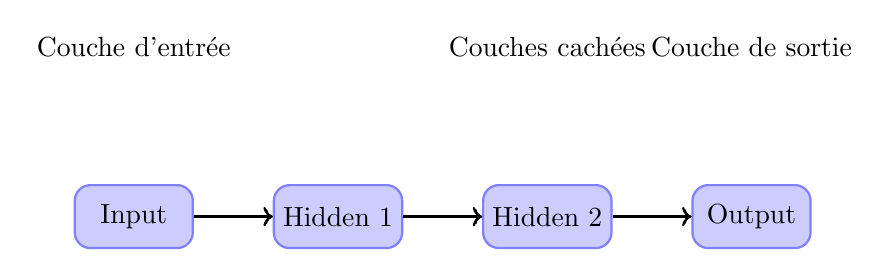
\begin{tikzpicture}[
    node distance=1.5cm and 1cm,
    layer/.style={rectangle, draw=blue!50, fill=blue!20, thick, minimum width=1.5cm, minimum height=0.8cm, rounded corners=0.2cm},
    neuron/.style={circle, draw=black, fill=gray!20, thick, minimum size=6mm}
]

% Input layer
\node[layer] (input) {Input};
\node[above=of input] (input_label) {Couche d'entrée};

% Hidden layers
\node[layer, right=of input] (hidden1) {Hidden 1};
\node[layer, right=of hidden1] (hidden2) {Hidden 2};
\node[above=of hidden2] (hidden_label) {Couches cachées};

% Output layer
\node[layer, right=of hidden2] (output) {Output};
\node[above=of output] (output_label) {Couche de sortie};

% Connect input to hidden1
\foreach \i in {1,...,3}
{
    \draw[->] (input) -- (hidden1);
}

% Connect hidden1 to hidden2
\foreach \i in {1,...,4}
{
    \draw[->] (hidden1) -- (hidden2);
}

% Connect hidden2 to output
\foreach \i in {1,...,2}
{
    \draw[->] (hidden2) -- (output);
}

% Arrows between layers
\draw[->, thick] (input) -- (hidden1);
\draw[->, thick] (hidden1) -- (hidden2);
\draw[->, thick] (hidden2) -- (output);

\end{tikzpicture}
\end{document}